\chapter{Imaging Radio Sources using CASA}

\section{Introduction}

CASA, or Common Astronomy Software Applications, is a suite of tools developed by the National Radio Astronomy Observatory (NRAO) to process radio interferometric data. It is a powerful tool that can be used to calibrate, image and analyze radio interferometric data. In this section, we will discuss how to use CASA to image radio sources.

% Inferometry

\subsection{Interferometry}

Interferometry is a technique used in radio astronomy to combine signals from multiple telescopes to form a single image. The basic idea behind interferometry is to use the interference pattern created by the combination of signals from multiple telescopes to reconstruct an image of the sky. The resolution of an interferometer is determined by the distance between the telescopes, with larger distances resulting in higher resolution images.

% CASA

\subsection{CASA}

CASA is a software package that is specifically designed to process radio interferometric data. It provides a wide range of tools for calibrating, imaging and analyzing radio interferometric data. CASA is widely used in the radio astronomy community and is the standard software package used for processing data from radio interferometers such as the Atacama Large Millimeter Array (ALMA) and the Very Large Array (VLA).

\clearpage

\section{TW Hydra}

In this section, we will use CASA to image the radio source TW Hydra. TW Hydra is a young star located in the constellation Hydra, approximately 176 light years from Earth. It is a popular target for radio observations due to its proximity and young age.

\subsection{`plotms' command}

The `plotms' command in CASA is used for UV data visualization. It can be used to plot visibility data from a measurement set and provides a range of options for customizing the plot. The `plotms' command is a useful tool for visualizing the visibility data and identifying any issues with the data.

\lstdefinestyle{casa-python}{
       language=Python,
       keywordstyle=\color{blue}\bfseries,
       commentstyle=\color{green},
       stringstyle=\color{red},
       numberstyle=\color[rgb]{0.205, 0.142, 0.73},
       basicstyle=\ttfamily\footnotesize,
       breaklines=true,
       frame=single,
       numbers=left,
       numberstyle=\tiny\color{gray},
       stepnumber=1,
       tabsize=4,
       showspaces=false,
       showstringspaces=false,
       showtabs=false,
       captionpos=b,
       morekeywords={vis, xaxis, yaxis, axis, avgchannel, avgspw, avgtime, avgscan, coloraxis, showgui, imagename, field, spw, specmode, deconvolver, gridder, imsize, cell, weighting, threshold, niter, interactive, width, outputvis, robust, datacolumn, mask}, % Add CASA-specific keywords if needed
       upquote=true,
}

\vspace{15mm}

\begin{lstlisting}[style=casa-python]
plotms(vis='sis14_twhya_calibrated_flagged.ms', 
       xaxis='u', 
       yaxis='v', 
       avgchannel='10000', 
       avgspw=False, 
       avgtime='1e9', 
       avgscan=False, 
       coloraxis="field", 
       showgui=True)
\end{lstlisting}

\begin{figure}[H]
	\centering
	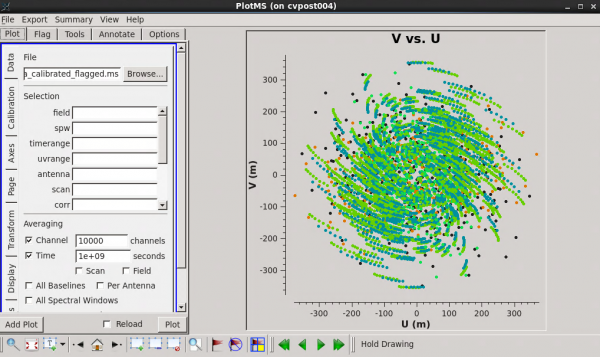
\includegraphics[width=0.8\textwidth]{Images/uv.png}
	\caption{Plot of visibility data for TW Hydra using the `plotms' command in CASA.}
\end{figure}

\clearpage

\subsection{`tclean' command}

The `tclean' command in CASA is used to image the radio source using the visibility data from a measurement set. The `tclean' command uses a deconvolution algorithm to reconstruct the image of the sky from the visibility data. The `tclean' command can be used to create high resolution images of radio sources.

\vspace{15mm}

\begin{lstlisting}[style=casa-python]
tclean(vis='sis14_twhya_calibrated_flagged.ms',
   imagename='phase_cal',
   field='3',
   spw='',
   specmode='mfs',
   deconvolver='hogbom',
   gridder='standard',
   imsize=[128,128],
   cell=['0.1arcsec'],
   weighting='briggs',
   threshold='0mJy',
   niter=5000,
   interactive=True)
\end{lstlisting}

\begin{figure}[H]
	\centering
	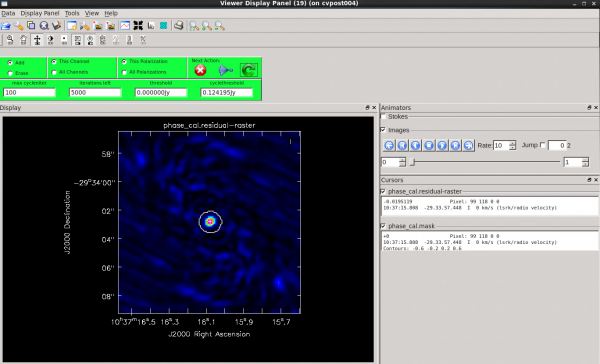
\includegraphics[width=0.8\textwidth]{Images/tclean.png}
	\caption{The tclean GUI showing the clean mask (white oval) circling the emission region.}
\end{figure}

\clearpage

\subsubsection{Using Briggs Weighing}

\begin{lstlisting}[style=casa-python]
tclean(vis='sis14_twhya_calibrated_flagged.ms',
       imagename='phase_cal_robust',
       field='3',
       spw='',
       specmode='mfs',
       gridder='standard',
       deconvolver='hogbom',
       imsize=[128,128],
       cell=['0.1arcsec'],
       weighting='briggs',
       robust=-1.0,
       threshold='0mJy',
       niter=5000,
       interactive=True)
\end{lstlisting}

\begin{figure}[H]
	\centering
	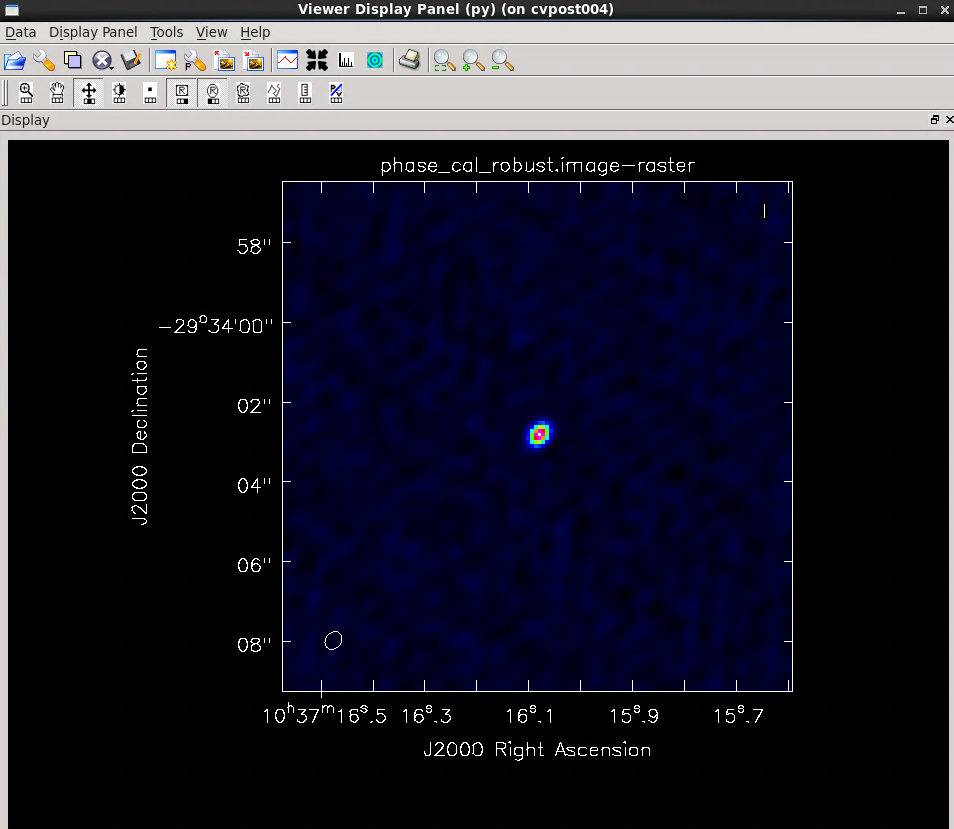
\includegraphics[width=0.8\textwidth]{Images/tclean-robust.png}
	\caption{Viewer image of the phase calibrator after tclean with briggs weighting.}
\end{figure}

\clearpage

\subsubsection{Increasing the Pixel size}

\begin{lstlisting}[style=casa-python]
tclean(vis='sis14_twhya_uncalibrated.ms',
       imagename='phase_cal_uncalibrated',
       field='3',
       spw='',
       specmode='mfs',
       gridder='standard',
       deconvolver='hogbom',
       imsize=[128,128],
       cell=['0.1arcsec'],
       weighting='natural',
       threshold='0mJy',
       niter=5000,
       interactive=True)
\end{lstlisting}

\begin{figure}[H]
       \centering
       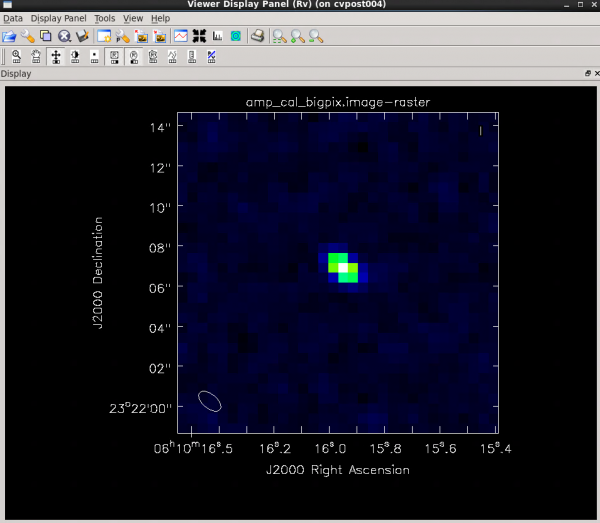
\includegraphics[width=0.8\textwidth]{Images/large-pixel-size.png}
       \caption{Viewer image of the amplitude calibrator after tclean with a large pixel size.}
\end{figure}

\clearpage

\subsubsection{Effects of Uncaliberated Data}

\begin{lstlisting}[style=casa-python]
tclean(vis='sis14_twhya_uncalibrated.ms',
       imagename='phase_cal_uncalibrated',
       field='3',
       spw='',
       specmode='mfs',
       gridder='standard',
       deconvolver='hogbom',
       imsize=[128,128],
       cell=['0.1arcsec'],
       weighting='natural',
       threshold='0mJy',
       niter=5000,
       interactive=True)
\end{lstlisting}

\begin{figure}[H]
       \centering
       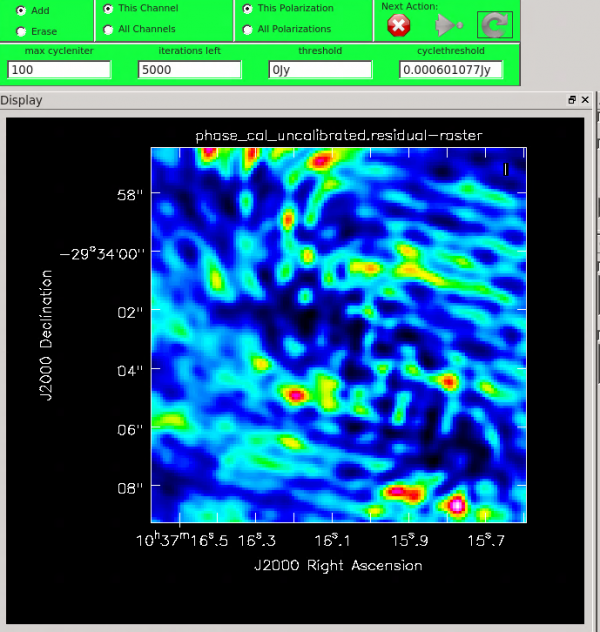
\includegraphics[width=0.8\textwidth]{Images/uncaliberated-image.png}
       \caption{Viewer image of the phase calibrator without any calibration.}
\end{figure}

\subsubsection{Effects of Unflagged Data}

\begin{lstlisting}[style=casa-python]
tclean(vis='sis14_twhya_calibrated.ms',
       imagename='phase_cal_unflagged',
       field='3',
       spw='',
       specmode='mfs',
       gridder='standard',
       deconvolver='hogbom',
       imsize=[128,128],
       cell=['0.1arcsec'],
       weighting='natural',
       threshold='0mJy',
       niter=5000,
       interactive=True)
\end{lstlisting}

\begin{figure}[H]
       \centering
       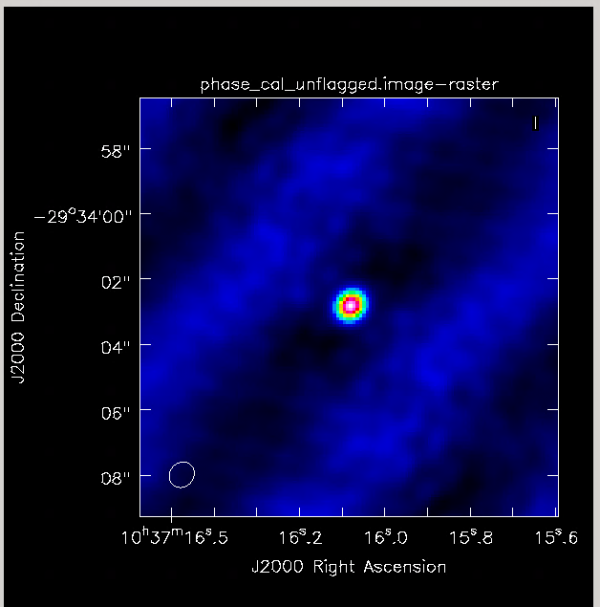
\includegraphics[width=0.8\textwidth]{Images/unflagged-image.png}
       \caption{Viewer image of the phase calibrator without any flagging of bad data.}
\end{figure}

\clearpage

\subsection{Continuum Image of TW Hydra}

\begin{lstlisting}[style=casa-python]
split(vis='sis14_twhya_calibrated_flagged.ms', field='5', width='8', outputvis='twhya_smoothed.ms', datacolumn='data')

tclean(vis='twhya_smoothed.ms',
       imagename='twhya_cont',
       field='0',
       spw='',
       specmode='mfs',
       gridder='standard',
       deconvolver='hogbom',
       imsize=[250,250],
       cell=['0.08arcsec'],
       weighting='briggs',
       robust=0.5,
       threshold='0mJy',
       niter=5000,
       interactive=True)
\end{lstlisting}

\begin{figure}[H]
       \centering
       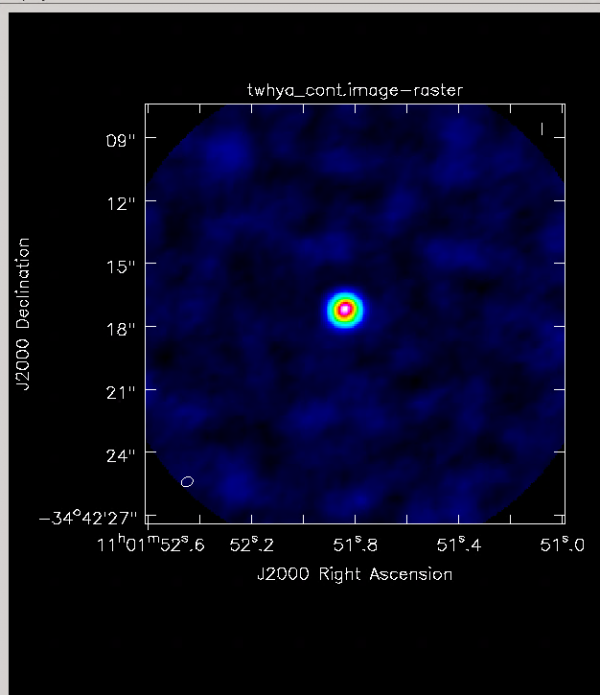
\includegraphics[width=0.7\textwidth]{Images/continuum-image.png}
       \caption{Continuum image for TW Hydra.}
\end{figure}

\clearpage

\subsection{Non-Interactive Cleaning Mode}

In the non-interactive mode of tclean, crucial parameters such as the threshold, mask, and maximum number of iterations play pivotal roles in controlling the deconvolution process. To set up tclean efficiently, first define a clean mask based on the regions of emission visible in the image. For instance, if emission is confined within a pixel range of $(100, 100)$ to $(150, 150)$, this box can be specified as the mask using the mask parameter. Alternatively, a mask file from an earlier interactive run can be used. Setting the stopping threshold involves estimating the noise level using tools like imview. In this scenario, an RMS noise of approximately $7$ mJy/beam suggests setting the threshold to about $15$ mJy/beam, which is twice the noise level. This approach helps to prevent the inclusion of random noise spikes as sources in the deconvolved image, thereby reducing false detections. \\

Additionally, the maximum number of iterations is set to $10,000$ as a failsafe measure. This high value ensures that tclean does not run indefinitely if something goes awry. The non-interactive mode of tclean offers a time-efficient and reproducible approach, though it is often advantageous to use the hybrid mode, starting interactively and then allowing tclean to continue automatically. This hybrid mode facilitates manual adjustments to the mask, threshold, and iteration parameters if necessary. For images with uncertain calibration or bright sources, an initial interactive cleaning process is recommended to ensure optimal results. Monitoring residuals during the cleaning cycles is essential, as increasing residuals may indicate the need for adjustments to the stopping threshold.

\vspace{15mm}

\begin{lstlisting}[style=casa-python]
tclean(vis='twhya_smoothed.ms',
       imagename='twhya_cont_auto',
       field='0',
       spw='',
       specmode='mfs',
       gridder='standard',
       deconvolver='hogbom',
       imsize=[250,250],
       cell=['0.08arcsec'],
       mask='box [ [ 100pix , 100pix] , [150pix, 150pix ] ]',
       weighting='briggs',
       robust=0.5,
       threshold='15mJy',
       niter=10000,
       interactive=False)
\end{lstlisting}